\chapter{Temperature as Energy and as the Derivative of Entropy}

This lecture unfolds in a deliberately careful order. We do not begin by defining temperature. We begin by removing the human conventions that make temperature look more mysterious than it is. Once temperature has been recast as an energy, and entropy as a dimensionless quantity, the statistical-mechanical definition can appear in its proper form. These notes follow Leonard Susskind's Lecture 2 closely, while preserving selected board images as documentary evidence; those visual materials are retained here with the help of LazyingArt LLC and Video2Book.

\section{Units, Conversion Factors, and Why Temperature Is Really Energy}

The lecture opens with a question that sounds elementary but is not: what is Boltzmann's constant? Susskind's answer is that \(k_B\) is, first of all, a conversion factor. In that respect it belongs to the same family as the speed of light. One may use \(c\) to convert distances into times; one uses \(k_B\) to convert human temperature units into energy units.

This is worth emphasizing because the ordinary temperature scales are historical constructions. Kelvin is measured from absolute zero, Celsius from the freezing and boiling points of water, and the size of a degree was chosen for convenience. Those units are perfectly useful, but they are not the units that microscopic physics would have invented from scratch.

The natural unit of temperature is energy. The lecture insists on this before anything else happens.

A dilute gas gives the cleanest example. The average kinetic energy of one molecule is
\begin{equation}
\langle E_{\mathrm{kin}}\rangle = \frac{3}{2} k_B T_{\mathrm{Kelvin}}.
\end{equation}
The factor of \(3\) comes from the three directions of space; the factor of \(1/2\) is the familiar one from kinetic energy. What matters here is that the combination \(k_B T_{\mathrm{Kelvin}}\) has units of energy.

Susskind then pushes the point with a slightly comic but very effective example. Put a bowling ball into a fluid in thermal equilibrium. Its speed will be tiny compared with that of a molecule, but its characteristic kinetic energy is set by the same temperature. Equal temperature does not mean equal velocity. It means equal energy scale.

For that reason we define a more fundamental temperature variable by
\begin{equation}
T := k_B T_{\mathrm{Kelvin}}.
\end{equation}
Now temperature is itself measured in energy units. The same kinetic-energy relation becomes
\begin{equation}
\langle E_{\mathrm{kin}}\rangle = \frac{3}{2} T.
\end{equation}

This is the first payoff of the lecture. Once temperature is written in fundamental units, \(k_B\) disappears from the formulas. It has not gone away physically. It has been absorbed into the choice of units.

There is also an important conceptual side remark here. The numerical value of \(k_B\) is not an absolute thing independent of convention. If one changed from Kelvin to some other temperature scale, the numerical value of \(k_B\) would change. That is precisely what conversion factors do.

\section{Entropy Units and the Disappearance of \texorpdfstring{$k_B$}{kB}}

Susskind then performs the same cleanup for entropy. Historically, entropy first appeared in thermodynamics in engineering units. Carnot did not know anything about microscopic states or information. He had a macroscopic quantity, useful for steam engines, with units of energy divided by temperature. If temperature is measured in Kelvin, that means joules per Kelvin.

Statistical mechanics uses a different normalization. For a discrete probability distribution \(\{p_i\}\), the entropy is
\begin{equation}
S = -\sum_i p_i \log p_i.
\end{equation}
This quantity is dimensionless. It is measured in the same sense that information is measured: one bit corresponds to \(\log 2\).

The lecture therefore distinguishes two entropies: Carnot's engineering entropy and Boltzmann's statistical entropy. Their relation is
\begin{equation}
S = \frac{1}{k_B} S_{\mathrm{Carnot}}.
\end{equation}
Equivalently,
\begin{equation}
S_{\mathrm{Carnot}} = k_B S.
\end{equation}

So the same constant \(k_B\) converts not only ordinary temperature into energy, but also engineering entropy into dimensionless entropy. Once both conversions have been made, the later formulas can be written in their cleanest form. This is why the long opening discussion of units is not a detachable preface. It prepares the ground for the relation
\[
dE = T\,dS
\]
so that when it finally appears it does not look like an arbitrary formal trick with a missing constant.

\begin{remark}
From this point on we write \(T\) for temperature in energy units and \(S\) for dimensionless statistical entropy. If one ever wants to go back to human units, one restores \(T = k_B T_{\mathrm{Kelvin}}\) and \(S_{\mathrm{Carnot}} = k_B S\).
\end{remark}

\section{Thermal Equilibrium as a Probability Distribution Over States}

Having cleared away the units, Susskind makes the sharp pivot: thus far he still has not told us what temperature is.

The next step is thermal equilibrium. Here the system should not be imagined as forever frozen in one exact microstate. Quite the opposite: the system may be exchanging energy with an environment, or heat bath, and its instantaneous energy may fluctuate. Thermal equilibrium means that after enough time the statistical description settles down. On the average, energy is flowing neither way.

Let the microscopic states of the system be labeled by \(i\), with energies \(E_i\). In equilibrium there is a probability \(P(i)\) that the system is in the \(i\)-th state. Those probabilities satisfy the normalization condition
\begin{equation}
\sum_i P(i)=1,
\end{equation}
and the average energy is
\begin{equation}
\sum_i P(i)E_i = E.
\end{equation}
On the board the same equation is written in a mixed notation as \(\sum_i P(i)E(i)=\langle E\rangle\). In these notes we standardize to \(E_i\) for the energy of the \(i\)-th state and \(E\) for the average energy.

\begin{figure}[t]
\centering

\includegraphics[width=0.78\textwidth]{lecture_02_figure_02.png}
\caption{Normalization and average energy. The board mixes \(E_i\), \(E(i)\), and \(\langle E\rangle\), but the content is the same: probabilities sum to one, and the weighted sum of state energies gives the average energy.}
\end{figure}

The word \emph{average} matters. The energy is not assumed to be sharply fixed at every instant. It fluctuates because the system exchanges energy with its surroundings. If one measures the system repeatedly, one gets a distribution of outcomes. The equilibrium quantity is the average of that fluctuating energy.

This is the first genuinely statistical description of equilibrium in the lecture. We are no longer talking about a thermometer reading in the abstract. We are talking about a probability distribution over microstates.

\section{A One-Parameter Family of Equilibrium Distributions}

Once the equilibrium probabilities have been introduced, the lecture asks the next question: what does the probability distribution depend on? The answer is that it depends, above all, on the average energy.

This is a physical statement before it is a formal one. Heat a pot of water on the stove, and you change its average energy. Cool it in the snow, and you change the average energy in the opposite direction. The equilibrium distribution changes with that parameter. So equilibrium is not one distribution but a family of them.

We therefore write
\begin{equation}
P(i,E),
\end{equation}
where the symbol \(E\) now labels the average energy of the distribution, not the energy \(E_i\) of an individual microscopic state.

For each member of the family, the defining relations are
\begin{align}
\sum_i P(i,E) &= 1, \\
\sum_i P(i,E)\,E_i &= E.
\end{align}
These are the cleaned-up equations that correspond to the board discussion. The board still shows the older unparameterized formulas on the left, but the spoken argument has already moved to the one-parameter family.

\begin{figure}[t]
\centering

\includegraphics[width=0.88\textwidth]{lecture_02_figure_03.png}
\caption{Setting up the probability distribution \(P(i,E)\). The board is in transition: earlier entropy and average-energy formulas remain on the left while the new graph appears on the right.}
\end{figure}

The lecture then shifts from formulas to pictures. On the right-hand side of the board Susskind draws axes labeled \(P(i,E)\). At first the horizontal variable may be thought of simply as the state label \(i\). But once the states are ordered by increasing energy, the same axis may also be read as tracking \(E_i\).

\begin{figure}[t]
\centering
\begin{tikzpicture}[scale=0.95]
\draw[->] (0,0) -- (0,3.1) node[left] {$P(i,E)$};
\draw[->] (0,0) -- (7.0,0) node[right] {$i$};
\end{tikzpicture}
\caption{A restrained reconstruction of the first graph. At this stage the horizontal axis may be read either as the state label \(i\) or, after ordering the states by energy, as a proxy for \(E_i\).}
\end{figure}

The important point is that equilibrium depends on a parameter. For each value of the average energy there is a different equilibrium distribution. The lecture does not derive that family yet; it takes it as a matter of experience and postpones the derivation of the Boltzmann distribution.

\subsection{Question \& Answer}

\paragraph{Question.} Isn't this circular? The average energy is computed from the probability distribution, but the probability distribution is now being labeled by the average energy.

\paragraph{Answer.} Susskind's answer is cautious and deliberately provisional. For the moment we assume that there is a one-parameter family of equilibrium distributions. Each distribution has an average energy. If no two members of the family have the same average energy, then the average energy can be used to label the family. The notation \(P(i,E)\) is therefore a convenient naming convention for a family that is being assumed, not yet derived.

Several classroom clarifications sharpen the point. First, Susskind says \emph{average} energy rather than \emph{total} energy because the system is imagined to be in contact with a heat bath, so its energy fluctuates. Second, to make the graph readable, he asks us to adopt a simple working assumption: label the states in increasing order of energy, and ignore exact degeneracies. That is why the horizontal axis may slide from a state label \(i\) to something like \(E_i\) without changing the logic of the picture.

\section{Entropy as a Function of Average Energy}

At this point the lecture inserts what Susskind calls ``one more thing.'' Each member of the family \(P(i,E)\) has its own entropy. Therefore entropy becomes a function of the average energy:
\begin{equation}
S(E) = -\sum_i P(i,E)\log P(i,E).
\end{equation}

This is not yet a universal function of energy. It depends on the particular family of equilibrium distributions for the system under discussion. But once the family has been granted, entropy is no longer an independent object floating beside it. It becomes a function built from that family.

That is the role of the next board picture. As the average energy increases, the probability distribution spreads and shifts to the right. The lecture is not yet calculating those distributions. It is using the sketch to make the dependence on average energy visible.

\begin{figure}[t]
\centering

\includegraphics[width=0.88\textwidth]{lecture_02_figure_04.png}
\caption{Different distributions with different average energies. The right-hand sketch is schematic, but it makes the lecture's point clearly: higher average energy shifts probability weight toward higher-energy states.}
\end{figure}

\begin{figure}[t]
\centering
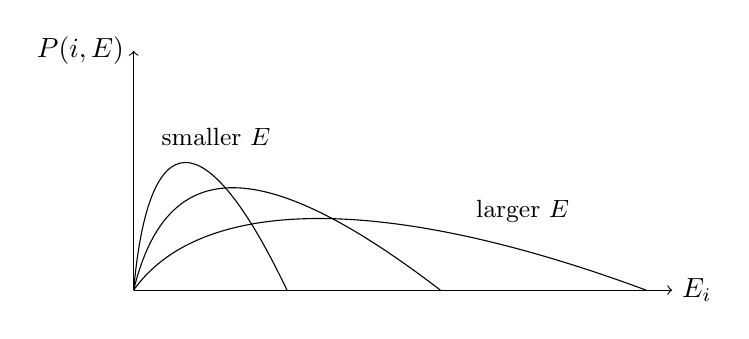
\begin{tikzpicture}[scale=0.95]
\draw[->] (0,0) -- (0,3.2) node[left] {$P(i,E)$};
\draw[->] (0,0) -- (7.2,0) node[right] {$E_i$};

\draw (0,0) .. controls (0.20,2.25) and (0.95,2.30) .. (2.05,0);
\draw (0,0) .. controls (0.45,1.85) and (1.75,1.80) .. (4.10,0);
\draw (0,0) .. controls (0.85,1.20) and (3.20,1.35) .. (6.85,0);

\node at (1.10,2.05) {\small smaller \(E\)};
\node at (5.20,1.05) {\small larger \(E\)};
\end{tikzpicture}
\caption{A cleaned reconstruction of the family \(P(i,E)\). Each curve represents an equilibrium distribution; increasing the average energy shifts the support toward higher-energy states.}
\end{figure}

The lecture does not yet prove that higher average energy always means higher entropy. It takes that as a typical feature of ordinary systems: when the distribution spreads over more states, entropy tends to increase. That working assumption will be important in a moment.

\section{Defining Temperature from the Entropy-Energy Derivative}

Now the lecture asks what Susskind himself calls a funny question: how much energy does it take to change the entropy by one bit?

At first the answer sounds almost disappointingly trivial. If energy is a smooth function of entropy, then
\begin{equation}
dE = \frac{dE}{dS}\, dS.
\end{equation}
Equally well one may write
\begin{equation}
dS = \frac{dS}{dE}\, dE.
\end{equation}
A student objects that perhaps \(dS/dE\) is the more natural quantity. Susskind's reply is that either form carries the same information: the two derivatives are inverses of one another when the function is single-valued.

The lecture then promotes the apparently trivial derivative into the central object:
\begin{definition}
Temperature is defined by
\begin{equation}
T = \frac{dE}{dS}.
\end{equation}
Equivalently,
\begin{equation}
dE = T\, dS,
\end{equation}
or
\begin{equation}
dS = \frac{1}{T}\, dE.
\end{equation}
\end{definition}

This is the universal definition the lecture wants us to remember. Temperature is a derived quantity. It measures how much energy must be added to produce a small increase in entropy.

The ``one bit'' question gives a concrete way to read the formula. If the entropy is changed by one bit, that is by \(\log 2\), then locally
\begin{equation}
\Delta E \approx T \log 2,
\end{equation}
provided the change is small enough that \(T\) may be treated as approximately constant over the step. That is not a new law; it is simply the differential relation read in a practical way.

There is also an important consistency check with the earlier unit conversion. Since
\begin{equation}
T = k_B T_{\mathrm{Kelvin}}, \qquad S = \frac{1}{k_B} S_{\mathrm{Carnot}},
\end{equation}
the fundamental relation becomes
\begin{equation}
dE = T_{\mathrm{Kelvin}}\, dS_{\mathrm{Carnot}}.
\end{equation}
The two factors of \(k_B\) cancel. This is why the same thermodynamic formula appears in ordinary textbooks without an explicit Boltzmann constant.

\subsection{Question \& Answer}

\paragraph{Question.} Why is it legitimate to regard \(S\) as a single-valued function of \(E\)? Is that obvious?

\paragraph{Answer.} It is not obvious, and the lecture says so explicitly. There are counterexamples. But for normal physical systems it is typically true that increasing the average energy broadens the equilibrium distribution and increases the entropy. For the purposes of this lecture we take that monotonicity as a working assumption. Under that assumption \(S(E)\) is single-valued, \(dS/dE\) and \(dE/dS\) make sense, and the temperature is positive.

This is the point at which the lecture pauses and says, in effect: we now have a definition of temperature, but it is still an abstract one. What does it have to do with the familiar notion of hot and cold? The answer comes from energy flow.

\section{Two Weakly Coupled Systems and the Direction of Energy Flow}

To recover the ordinary meaning of temperature, Susskind considers two systems, \(A\) and \(B\), initially each in equilibrium but at different temperatures. They are connected by a thin pipe. The pipe is thin in the thermodynamic sense: the systems can exchange energy, but only weakly, so that each still makes sense as a subsystem with its own entropy and temperature.

Let the initial temperatures satisfy
\begin{equation}
T_B > T_A.
\end{equation}
Which way will the energy flow? The familiar answer is from hot to cold. The lecture now shows that this familiar fact is encoded in the derivative definition of temperature.

Three ingredients are assembled.

First, the total entropy is additive:
\begin{equation}
S_{\mathrm{tot}} = S_A + S_B.
\end{equation}
In the lecture this is justified heuristically by the fact that entropy is the logarithm of a multiplicative quantity.

Second, the total energy is conserved:
\begin{equation}
dE_A = -\,dE_B.
\end{equation}
This is the first law in the present setting.

Third, the second law says that during equilibration the total entropy increases:
\begin{equation}
dS_A + dS_B > 0.
\end{equation}

Now use the definition of temperature separately for each subsystem:
\begin{equation}
dE_A = T_A\, dS_A,
\qquad
dE_B = T_B\, dS_B.
\end{equation}
Therefore
\begin{equation}
dS_A = \frac{dE_A}{T_A},
\qquad
dS_B = \frac{dE_B}{T_B}.
\end{equation}
Substituting into the total entropy change gives
\begin{align}
dS_{\mathrm{tot}}
&= dS_A + dS_B \\
&= \frac{dE_A}{T_A} + \frac{dE_B}{T_B} \\
&= \frac{dE_A}{T_A} - \frac{dE_A}{T_B} \\
&= dE_A\left(\frac{1}{T_A} - \frac{1}{T_B}\right).
\end{align}

Now suppose \(T_B > T_A\). Then
\begin{equation}
\frac{1}{T_A} - \frac{1}{T_B} > 0.
\end{equation}
Since the second law requires \(dS_{\mathrm{tot}} > 0\), it follows that
\begin{equation}
dE_A > 0.
\end{equation}
So system \(A\) gains energy while system \(B\) loses it. Energy flows from \(B\), the hotter system, to \(A\), the colder one.

If instead \(T_A = T_B\), then the coefficient vanishes and there is no preferred direction of flow. That is the equilibrium condition for the composite system.

\begin{remark}
The transcript becomes ragged before the final sign argument is fully written out, but the computation above is the minimal cautious completion of the equations Susskind explicitly sets up: entropy additivity, total-energy conservation, the second law, and \(dE = T\,dS\) for each subsystem.
\end{remark}

The abstract derivative has now recovered the ordinary physical meaning. Temperature is precisely the quantity whose difference determines the direction of spontaneous energy flow.

\section{Summary}

The lecture begins by refusing to define temperature too quickly. First we are asked to stop thinking in human units. Boltzmann's constant is only a conversion factor: it converts thermometer temperature into energy, and engineering entropy into dimensionless statistical entropy. Once those conversions are made, the formulas simplify and \(k_B\) may be suppressed.

Only then does the statistical-mechanical structure emerge. A system in equilibrium is described by probabilities \(P(i)\) over microscopic states \(i\), with average energy
\[
\sum_i P(i)E_i = E.
\]
Equilibrium is then recast as a one-parameter family \(P(i,E)\), and each member of that family has its own entropy
\[
S(E) = -\sum_i P(i,E)\log P(i,E).
\]

From that family comes the central derivative
\[
T = \frac{dE}{dS},
\]
or \(dE = T\,dS\). At first it looks like a trivial identity. Then the lecture reveals that it is the universal definition of temperature. Finally, by coupling two systems weakly and invoking the first and second laws, the lecture shows that this derivative is exactly what governs the flow of energy from hot to cold. The familiar notion of temperature is thus rebuilt from probability, entropy, and energy.